%%%%%%%%%%%%%%%%%%%%%%%%%%%%%%%%%%%%%%%%%
% Beamer Presentation
% LaTeX Template
% Version 1.0 (10/11/12)
%
% This template has been downloaded from:
% http://www.LaTeXTemplates.com
%
% License:
% CC BY-NC-SA 3.0 (http://creativecommons.org/licenses/by-nc-sa/3.0/)
%
%%%%%%%%%%%%%%%%%%%%%%%%%%%%%%%%%%%%%%%%%

%----------------------------------------------------------------------------------------
%	PACKAGES AND THEMES
%----------------------------------------------------------------------------------------

\documentclass{beamer}

\mode<presentation> {

% The Beamer class comes with a number of default slide themes
% which change the colors and layouts of slides. Below this is a list
% of all the themes, uncomment each in turn to see what they look like.

%\usetheme{default}
%\usetheme{AnnArbor}
%\usetheme{Antibes}
%\usetheme{Bergen}
%\usetheme{Berkeley}
%\usetheme{Berlin}
%\usetheme{Boadilla}
%\usetheme{CambridgeUS}
%\usetheme{Copenhagen}
%\usetheme{Darmstadt}
%\usetheme{Dresden}
%\usetheme{Frankfurt}
%\usetheme{Goettingen}
%\usetheme{Hannover}
%\usetheme{Ilmenau}
%\usetheme{JuanLesPins}
%\usetheme{Luebeck}
\usetheme{Madrid}
%\usetheme{Malmoe}
%\usetheme{Marburg}
%\usetheme{Montpellier}
%\usetheme{PaloAlto}
%\usetheme{Pittsburgh}
%\usetheme{Rochester}
%\usetheme{Singapore}
%\usetheme{Szeged}
%\usetheme{Warsaw}

% As well as themes, the Beamer class has a number of color themes
% for any slide theme. Uncomment each of these in turn to see how it
% changes the colors of your current slide theme.

%\usecolortheme{albatross}
%\usecolortheme{beaver}
%\usecolortheme{beetle}
%\usecolortheme{crane}
%\usecolortheme{dolphin}
%\usecolortheme{dove}
%\usecolortheme{fly}
%\usecolortheme{lily}
%\usecolortheme{orchid}
%\usecolortheme{rose}
%\usecolortheme{seagull}
%\usecolortheme{seahorse}
%\usecolortheme{whale}
%\usecolortheme{wolverine}

%\setbeamertemplate{footline} % To remove the footer line in all slides uncomment this line
%\setbeamertemplate{footline}[page number] % To replace the footer line in all slides with a simple slide count uncomment this line

%\setbeamertemplate{navigation symbols}{} % To remove the navigation symbols from the bottom of all slides uncomment this line
}

\usepackage{graphicx} % Allows including images
\usepackage{booktabs} % Allows the use of \toprule, \midrule and \bottomrule in tables
\usepackage[utf8]{inputenc}

%----------------------------------------------------------------------------------------
%	TITLE PAGE
%----------------------------------------------------------------------------------------

\title[AP3]{Detecção de Alertas de Segurança em Redes de Computadores Usando
o Internet Relay Chat}

\author{Daniel Bucher} % Your name
\institute[USP] % Your institution as it will appear on the bottom of every slide, may be shorthand to save space
{
Universidade de São Paulo \\ % Your institution for the title page
\medskip
\textit{dbucher@ime.usp.br} % Your email address
}
\date{\today} % Date, can be changed to a custom date

\begin{document}

\begin{frame}
\titlepage % Print the title page as the first slide
\end{frame}

\begin{frame}
\frametitle{Agenda}

\begin{enumerate}
    \item{IRC}
    \item{Objetivos do trabalho}
    \item{Desafios}
    \item{\textit{Toolkit} para análise de conversas de chat}
    \item{IRC Bot}
    \item{Tarefas futuras}
    \item{Referência}
\end{enumerate}
\end{frame}

%----------------------------------------------------------------------------------------
%	PRESENTATION SLIDES
%----------------------------------------------------------------------------------------
\begin{frame}
\frametitle{Internet Relay Chat}

O Internet Relay Chat (\textbf{IRC}), é um protocolo da \textbf{camada de aplicação} para transferência de texto. Ele funciona em uma \textbf{arquitetura
cliente-servidor}. Ele foi projetado pra conversas em grupo em salas de chat,
chamadas de \textbf{canais}.

\end{frame}

\begin{frame}
\frametitle{Internet Relay Chat}
\framesubtitle{História}

  \begin{itemize}
    \setlength\itemsep{0.8em}
    \item O IRC foi criado em 1988 por Jarkko Oikarinen, na Finlândia.
    \item O IRC vem perdendo força devido à popularização das redes sociais.
    \item Chegou a ter 1 milhão de usuários em 2003. Hoje tem cerca de 40\%
    disso.
    \item Chegou a ter meio milhão de canais em 2003. Hoje tem cerca de 50\%
    disso.
  \end{itemize}

\end{frame}

\begin{frame}
\frametitle{Internet Relay Chat}
\framesubtitle{Informações técnicas}

  \begin{itemize}
    \item O IRC utiliza conexões TCP, e opcionalmente, TLS.
    \item Um servidor IRC pode se conectar a outros servidores IRC, e assim
    expandir a rede.
    \item A \textbf{IANA} designou a porta \textbf{194/TCP} para ser usada por
     servidores IRC, no entanto, o padrão mais dissenimado é usar a porta
     \textbf{6667/TCP} para evitar ter de rodar o servidor com privilégio de
     root.
    \item A implementação original de um servidor IRC é chamada de
    \textbf{IRCd}.
    \item A implementação oficial do servidor atual de IRC é chamada de IRC2
    e está em sua versão 2.10.
  \end{itemize}

\end{frame}

\begin{frame}
\frametitle{Internet Relay Chat}
\framesubtitle{RFC}

  \begin{itemize}
    \setlength\itemsep{1em}
    \item RFC original: \textbf{RFC 1459}.
    \item Arquitetura do IRC: \textbf{RFC 2810}
    \item Gerenciamento de canais: \textbf{RFC 2811}
    \item Protocolo do cliente: \textbf{RFC 2812}
    \item Lado servidor atual: \textbf{RFC 2813}
  \end{itemize}

\end{frame}


%----------------------------------------------------------------------------------------

\begin{frame}
\frametitle{Objetivos do trabalho}

\begin{itemize}
    \setlength\itemsep{1.5em}
    \item Monitorar canais do IRC para verificar se estes possuem informações
    importantes sobre alertas de segurança de redes de computadores.
    \item Vericar se é possível extrair automaticamente esses alertas em canais
    do IRC.
\end{itemize}

\end{frame}

%-------------------------------------------------------------------------------

\begin{frame}
\frametitle{Desafios}

\begin{itemize}
    \setlength\itemsep{1.5em}
    \item A captura de mensagens que possuem palavras chave não fornece
    contexto.
    \item As ferramentas de processamento de linguagem natural, por padrão,
    não fornecem mecanismos para lidar com a estrutura temporal que conversas
    em chat possuem.
    \item É comum usuários de chat usarem uma linguagem informal nesses canais
    de comunicação.
\end{itemize}

\end{frame}

%-------------------------------------------------------------------------------

\begin{frame}
\frametitle{\textit{Toolkit} para análise de conversas de chat}
\framesubtitle{Arquitetura}

\begin{figure}
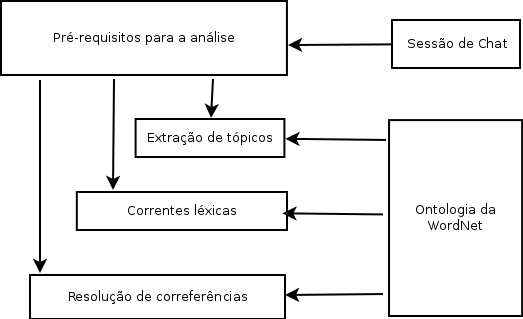
\includegraphics[width=0.6\linewidth]{gainaru_architecture.png}
\end{figure}

Arquitetura do \textit{toolkit} para análise de conversas de chat apresentado
por Gainaru et. al. (2010).

\end{frame}

%-------------------------------------------------------------------------------

\begin{frame}
\frametitle{Toolkit para análise de conversas de chat}
\framesubtitle{Pré requisitos para análise}

Realiza as atividades de:
\begin{itemize}
  \setlength\itemsep{0.8em}
  \item{\textit{Tokenização}}
  \item{Eliminação de palavras irrelevantes} (ex: `:)')
  \item{\textit{Word stemming}}
  \item{\textit{Part of Speech Tagging}}
\end{itemize}
\end{frame}

%-------------------------------------------------------------------------------

\begin{frame}
\frametitle{Toolkit para análise de conversas de chat}
\framesubtitle{Extração de tópicos}

\begin{itemize}
  \setlength\itemsep{1.2em}
  \item{Análise de frequência}
  \item{Agrupamento de sinônimos}
  \item{O resultado é a lista de tópicos}
\end{itemize}
\end{frame}

%-------------------------------------------------------------------------------

\begin{frame}
\frametitle{Toolkit para análise de conversas de chat}
\framesubtitle{Correntes léxicas e resolução de correferência}

\begin{itemize}
  \setlength\itemsep{1.2em}
  \item O terceiro módulo identifica correntes léxicas no texto. Uma corrente
  léxica é uma lista de palavras que captura uma porção da estrutura
  coerente  do texto.
  \item O quarto e último módulo analisa o texto em busca de correferências de
  termos não verbais (ex: ``\textbf{João} saiu de casa. \textbf{Ele} não voltou'')
\end{itemize}
\end{frame}

%-------------------------------------------------------------------------------

\begin{frame}
\frametitle{IRCBot}

\begin{itemize}

\item Para criarmos o bot que extrai as mensagens do IRC, utilizamos a
biblioteca \textbf{Cinch}, em Ruby.

\item O bot captura mensagens que possuam uma ou mais palavras chave.

\item Paralelamente, o bot registra todas as mensagens e eventos de entrada e
saída de usuário em um log do canal.

\item Dessa forma, ao identificarmos uma frase com uma palavra chave, podemos
capturar as mensagens anteriores e posteriores e extrair o contexto.
\end{itemize}

\end{frame}

%----------------------------------------------------------------------------------------

\begin{frame}
\frametitle{Tarefas futuras}

\begin{itemize}
  \item Identificar manualmente alguns exemplos de conversas que possuam
  alertas de segurança de redes de computadores.
  \item Identificar a partir das conversas do item anterior, um
  \textit{threshold} de mensagens anteriores e posteriores necessárias
  para minimizar a perda de contexto.
  \item Propor uma metodologia utilizando as técnicas de análise de texto
  de Gainaru et. al. (2010) para identificar, através dos tópicos da conversa
  se esta consiste em um alerta de segurança.
\end{itemize}

\end{frame}

%------------------------------------------------

\begin{frame}
\frametitle{Obrigado}

\Huge{\centerline{Dúvidas?}}
\end{frame}

%----------------------------------------------------------------------------------------

\begin{frame}
  \frametitle{References}
  \footnotesize{
  \begin{thebibliography}{99} % Beamer does not support BibTeX so references must be inserted manually as below
    \bibitem[IRC]{p1} Internet Relay Chat (2014)
    \newblock \emph{http://www.irc.org}

    \bibitem[Gainaru, 2013]{p2} A. Gainaru, S. D. Dumitrescu, S. Trausan-Matu (2010)
    \newblock Toolkit for automatic analysis of chat conversations
    \newblock \emph{``Politehnica'' University of Bucharest}
    
    \bibitem[Campiolo et. al., 2013]{p1} L. A. F. Santos and R. Campiolo and M. A. Gerosa and D. M. Batista (2013)
    \newblock Detecção de Alertas de Segurança em Redes de Computadores Usando Redes Sociais
    \newblock \emph{31º Simpósio Brasileiro de Redes de Computadores e Sistemas Distribuídos}

    \bibitem[Michels, 2013]{p2} M. O. Michels (2013)
    \newblock Real Time Text Analysis on Internet Relay Chat Conversations
    \newblock \emph{Center for Education and Research Information Assurance and Security, Purdue University}

  \end{thebibliography}
  }
\end{frame}

%----------------------------------------------------------------------------------------

\end{document}
